%!TEX root = Thesis.tex

\chapter{Clustering}


\section{The problem of clustering}
\label{sec:clustering}

%this is mostly taken from Jain's 50 years beyond K-Means
Advances in technology allow for the collection and storage unprecedented amount and variety of data.
Since data is mostly stored electronically, it presents a potential for automatic analysis and thus creation of information and knowledge.
A growing body of statistical methods aiming to model, structure and/or classify data already exist, e.g. linear regression, principal component analysis, cluster analysis, support vector machines, neural networks.
Many of these methods fall into the realm of machine learning, which is usually divided into 2 major groups: \textit{supervised} and \textit{unsupervised} learning.
% TODO: add some reference for the 2 major groups; optional: explain what learning is
Supervised learning deals with labeled data, i.e. data for which ground truth is known, and tries to solve the problem of classification. %TODO: add ref for solving classification
Unsupervised learning deals with unlabeled data and tries to solve the problem of clustering. % TODO: add ref for solving clustering

Cluster analysis is the backbone of the present work.
The goal of data clustering, as defined by \cite{Jain2010}, is the discovery of the \textit{natural grouping(s)} of a set of patterns, points or objects.
In other words, the goal of data clustering is to discover structure on data.
And the methodology used is to group patterns that are similar by some metric (e.g. euclidean distance, Pearson correlation) and separate those that are dissimilar. %TODO reference for a method for both euclidean distance and Pearson correlation

As an example, Figure \ref{fig:intro raw} shows the plot of a simple synthetic dataset - a Gaussian mixture of 5 distributions.
No extra information other than the position of the points is given, since clustering algorithms are unsupervised methods.
Figure \ref{fig:intro natural} presents the desired (or "natural") clustering for this given dataset.
Figure \ref{fig:intro kmeans} presents the clusters given by the K-Means algorithm with an initialization of 4 clusters.
The number of clusters was purposefully set to an "incorrect" number to demonstrate that the number of cluster of a dataset is not trivial to discover, even in such a simple example.
In this synthetic dataset, the number of clusters is not clear due to the two superimposed Gaussians.
The number of clusters is a common initialization parameter for clustering methods.
When no prior information about the dataset is given, the number of clusters can be hard to discover.

%TODO change this 3 plots to a three plot subfigure, with the plots side by side
% \begin{figure}[hbtp]
% \centering
% 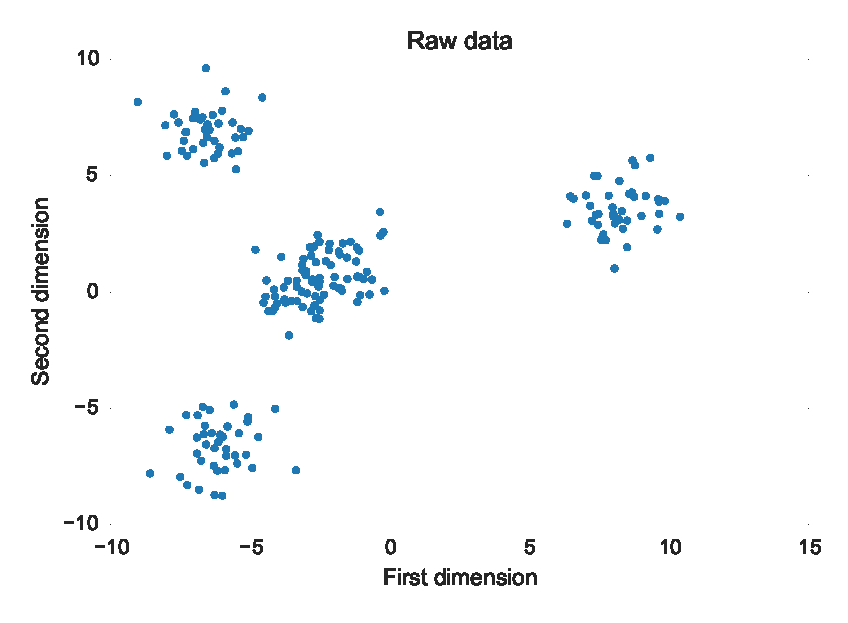
\includegraphics[scale=0.5]{introduction/img/cluster_example_raw.eps}
% \caption{Gaussian mixture of 5 distributions. The middle "ball" of points is 2 Gaussians that intersect.}
% \label{fig:intro raw}
% \end{figure}

% \begin{figure}[hbtp]
% \centering
% 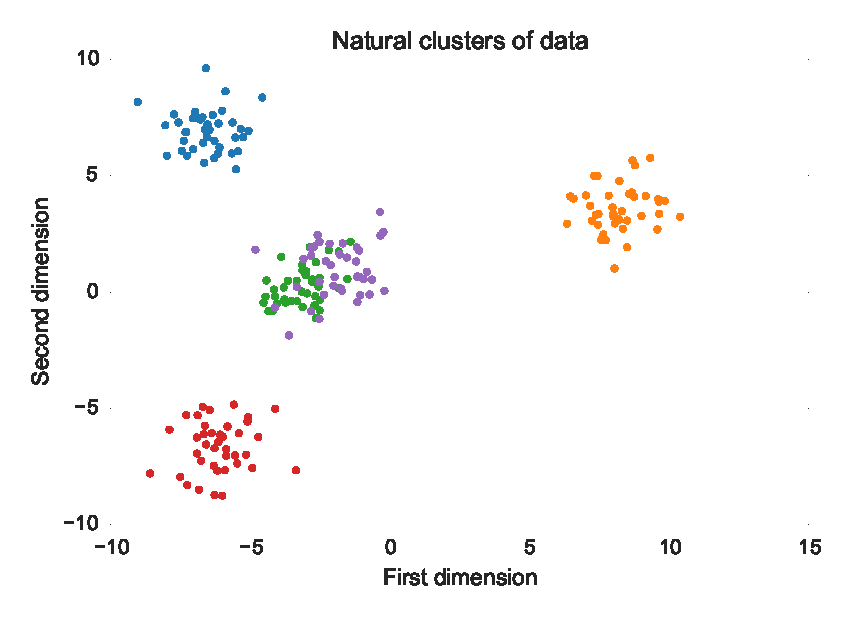
\includegraphics[scale=0.5]{introduction/img/cluster_example_natural.eps}
% \caption{Gaussian mixture of 5 distributions. The colors of each point represents the group (the Gaussian distribution) to which it belongs.}
% \label{fig:intro natural}
% \end{figure}

% \begin{figure}[hbtp]
% \centering
% 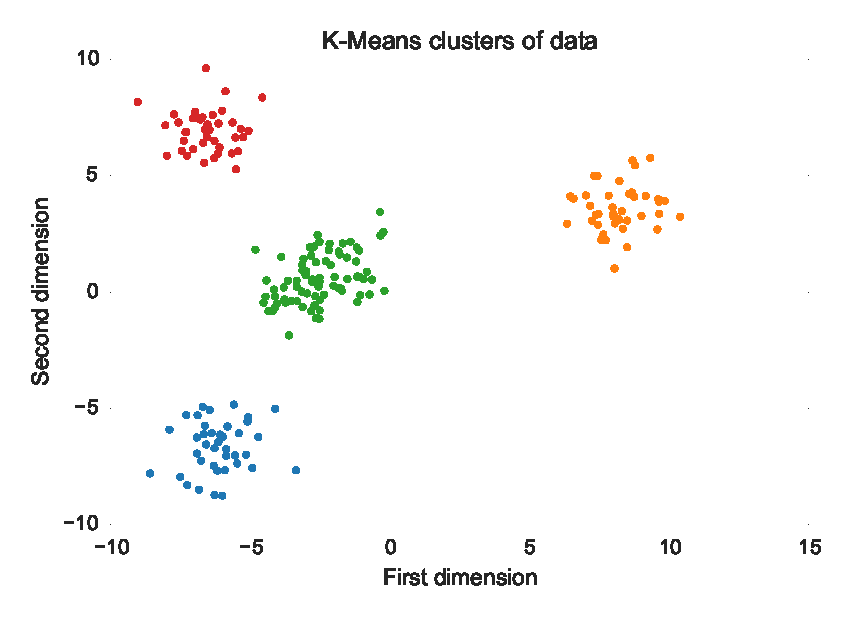
\includegraphics[scale=0.5]{introduction/img/cluster_example_kmeans.eps}
% \caption{Sama data, as Figure \ref{fig:intro raw}, but the group to which each point belongs to was computed by the K-Means algorithm with the number of clusters set to 4.}
% \label{fig:intro kmeans}
% \end{figure}

\begin{figure}[!ht]
    \centering
    \begin{subfigure}[b]{0.3\textwidth}
        \centering
        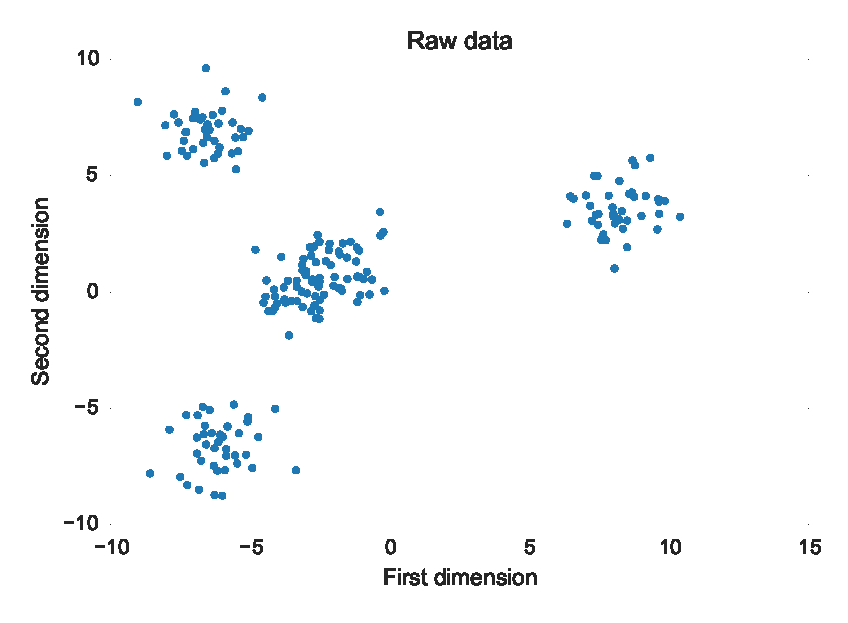
\includegraphics[width=\textwidth]{introduction/img/cluster_example_raw}
        \caption{Input data, unlabeled.}
        \label{fig:intro raw}
    \end{subfigure}
    \hfill
    \begin{subfigure}[b]{0.3\textwidth}
        \centering
        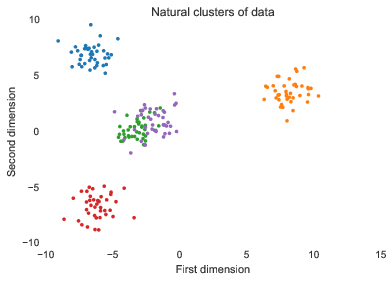
\includegraphics[width=\textwidth]{introduction/img/cluster_example_natural}
        \caption{Desired labels.}
        \label{fig:intro natural}
    \end{subfigure}
    \hfill
    \begin{subfigure}[b]{0.3\textwidth}
        \centering
        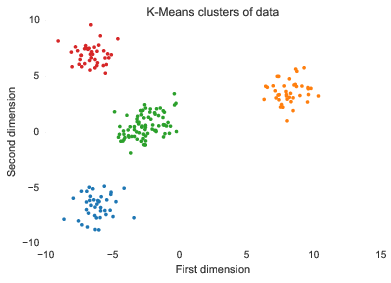
\includegraphics[width=\textwidth]{introduction/img/cluster_example_kmeans}
        \caption{K-Means's labels.}
        \label{fig:intro kmeans}
    \end{subfigure}
    \caption{Gaussian mixture of 5 distributions. Fig. \ref{fig:intro raw} shows the raw input data, i.e. how the algorithms "sees" the data. Fig. \ref{fig:intro natural} shows the desired labels for each point, which here means their corresponding Gaussian. Fig. \ref{fig:intro kmeans} shows the output labels of the K-Means algorithm with the number of clusters (input parameter) set to 4.}
    \label{fig:clustering plots}
\end{figure}


Cluster analysis is a relevant technique across several domains (\cite{Aggarwal2014}):

\begin{itemize}
	\item grouping users with similar behaviour or preferences in \textbf{customer segmentation};
	\item image segmentation in the field of \textbf{image processing};
	\item clustering gene expression data, among other application, in the domain of \textbf{biological data analysis};
	\item generation of hierarchical structure for easy access and retrieval of \textbf{information systems}; % not referenced in book
\end{itemize}

% Clustering is used in a wide variety of fields to solve numerous problems, e.g.:
% %TODO provide references to all of this
% % see https://sites.google.com/site/dataclusteringalgorithms/clustering-algorithm-applications
% % has applications with articles
% \begin{itemize}
% \item image segmentation in the field of image processing;
% \item generation of hierarchical structure for easy access and retrieval of information systems;
% \item recommender systems by grouping users by their behaviour and/or preferences;
% \item clustering customers for targeted marketing in 
% \item clustering gene expression data in biology;
% \item grouping of 
% \end{itemize}